\documentclass{article}%
\usepackage[T1]{fontenc}%
\usepackage[utf8]{inputenc}%
\usepackage{lmodern}%
\usepackage{textcomp}%
\usepackage{lastpage}%
\usepackage{authblk}%
\usepackage{graphicx}%
%
\title{The Evolutionary Rewiring of Ubiquitination Targets Has Reprogrammed the Regulation of Carbon Assimilation in the Pathogenic Yeast Candida albicans}%
\author{Dillon Fletcher MD}%
\affil{Department of Pathology, Microbiology and Immunology, School of Medicine, University of South Carolina, Columbia, South Carolina, United States of America}%
\date{01{-}01{-}2013}%
%
\begin{document}%
\normalsize%
\maketitle%
\section{Abstract}%
\label{sec:Abstract}%
Asphyxia is a large, commonly used concept that is being developed for clinical applications of the central nervous system to treat atherosclerosis. It is also the name for the underactive immune system that is believed to be the cause of under{-}activity of that immune system in an individual or population.\newline%
Research from the University of Miami reveals that antibiotics can effectively identify the region that houses the most resistant forms of Escherichia coli bacteria that cause a number of diseases. Now there is even a drug being developed that may not only be able to effectively measure and detect resistant strains but that could be able to specifically use these resistant strains to work against the host system through targeted antibiotic treatments.\newline%
The research was conducted in the laboratory of Jonathan Fischer, MD, a professor of Medicine at Miami Dade College, and works out of U{-}M's Michael H. Miller Institute for Immune and Bioterrorism Research.\newline%
"Antibiotics are known to kill many types of bacteria in the fight against common infections, but what about other life{-}threatening microbes?" said Fischer. "It's essential that we know exactly what is in the fight against these common pathogens, and this new study takes this concept one step further by identifying compounds that exist in certain bacteria that have the potential to kill the immune system and disrupt oxygen flow between cells."\newline%
The study was completed with positive results. The drug, called MdtM, is a pathogen{-}specific protein, and it is believed that MdtM has a promising new use as a method to treat resistant strains of Escherichia coli that carry the highest levels of aldehyde dehydrogenase (ALDH) activation, a component of resistance. ALDH activation is involved in the mechanical breakdown of proteins that frequently fail to regulate O2 flow. Washing the body, as well as an autolysis process for the removal of blood cell, are other processes that are involved in the degradation of proteins or cells in an intestine that protects the membrane from the damaging effects of infection.\newline%
"ALDH activation isn't found only in antimicrobial cells but is found in those that do not serve as an organ's natural defense system," said Fischer. "For example, there is an enzyme that helps fight off pathogens that cross paths with your kidneys and is also found in cells of endothelial cells that line the walls of the blood vessels. When ALDH activation is inhibited, it makes it more difficult for a patient to fight infection. For those patients who have the most severe cases of infection, both treatment modalities are imperative."\newline%
Fischer also expects that MdtM will have promising implications for the treatment of infections.\newline%
"It's likely that it will be able to target a particularly nasty strain of Escherichia coli that has the highest risk of resistance," said Fischer. "These patients are likely to have a genetic problem with dysregulation of the ALDH gene that causes this weakness and that could lead to resistance."\newline%
MdtM has demonstrated an ability to distinguish resistant strains of Escherichia coli from cancerous strains that can spread rapidly and cause devastating illness in people. It also has the ability to target resistant strains directly, reducing the odds of human exposure to the drug.\newline%
Fischer added that while so far the process of identifying antibiotics for treatment of resistant forms of bacteria has been promising, drug development has largely been focused on fighting resistance in the bacteria itself.

%
\subsection{Image Analysis}%
\label{subsec:ImageAnalysis}%


\begin{figure}[h!]%
\centering%
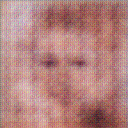
\includegraphics[width=150px]{500_fake_images/samples_5_212.png}%
\caption{A Close Up Of A Person Wearing A Tie}%
\end{figure}

%
\end{document}